\newpage
\section{Data}
\label{chapter:data}

% SECTIONS
% Experimental details
% Properties (preprocessing, cycles, confounding, …)
% Relevance; state-of-the-art
% Description of data subsets

\subsection{Data Source}

We evaluate our methods on a biological dataset. The DNA of a cell contains genes that are involved in many of the cell's functions. They are typically responsible for the production of a protein. The first step in this process is to copy its information to a Messenger RNA (mRNA) strand. The amount of mRNA that is measured in an experiment indicates how active a specific gene is, or how high its \textit{expression level}.

Genes interact to fulfill a plethora of cell functions. For example, the expression of one gene might up- or down-regulate the expression of some other gene. This interaction is regulated by biochemical processes. 

For a variety of reasons, it is interesting to know how genes interact precisely, that is: what the regulatory network looks like. By jointly measuring the expression of a large set of mRNA strands we obtain an mRNA profile. Collecting a set of these profiles allows us to model the joint distribution of mRNA expression and the causal relations among them.

Specifically, we use mRNA profiles from \citet{kemmeren2014large}. They measured a profile of 6.182 genes in cells of the yeast species \textit{Saccharomyces cerevisiae} (baker's yeast), using DNA microarray technology (Figure \ref{fig:3:microarray}). The dataset consists of 262 observation samples obtained from unaltered \textit{wild type} cells, and 1.484 intervention samples obtained from \textit{mutant} cells where one gene was deactivated\footnote{We use an earlier version of the dataset with 1.479 intervention genes.}.

\begin{figure}[h]
    \centering
    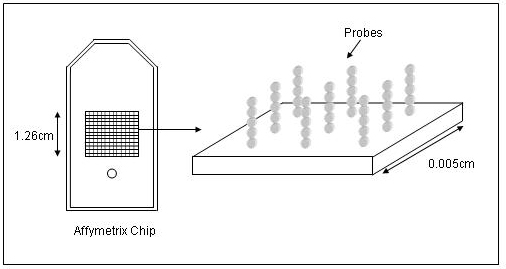
\includegraphics[width=.7\textwidth]{3microarray}
    \caption{Illustration of a typical microarray chip. Every small square can be used for an experiment to measure gene expression levels.\protect\footnotemark}
    \label{fig:3:microarray}
\end{figure}
\footnotetext{Source: http://grf.lshtm.ac.uk/microarrayoverview.htm}

Both the observational and interventional profiles are reported relatively to some average wild type profile. \citet{kemmeren2014large} report that the intervention profiles are compared to a set of 428 wild type profiles. Gene expression is measured as fluorescent intensity in the experiments. In this thesis, we work with the difference in $log_2$ fluorescent intensity between the data point and the reference wild type data, which indicates deviation from the normal gene expression levels. Because the data already indicates values relative to a norm, we choose to not preprocess the data.

% \silvan{It is unclear if the observational profiles are compared to the same set.} \silvan{ADD: measured as log2 fluorescent intensity} \silvan{ADD: some genes were excluded because they changed significantly in the WT already? see kemm. \textit{Statistical Analysis of Expression Profiles}}

There are some details of the experiments that might be of relevance in a discussion of underlying assumptions. First of all, the researchers chose to measure only a subset of about 25\% of all genes. Selection criteria included whether genes were expected to be involved in regulating other genes, and only genes were selected that do not play a vital role in keeping the cell alive (viability). 

Furthermore, the profile resulting from an experiment had to pass a quality control before being admitted to the dataset. Failing this test resulted either in repeating the experiment, or excluding the mutant. Although these checks improve the quality of the data by removing some failed experiments, they may admit some selection bias as well. 

Another form of selection bias is inherent in the experimental method. The mutant cells need to reproduce many times until a culture is grown that is large enough to do the measurements. However, cells with certain properties may reproduce quicker or easier, and be overrepresented in the measurement. It is unclear how large this effect may be.

A final factor to consider is that  data from previous work of the same institute is included in the dataset, specifically from \citet{lenstra2011specificity} and \citet{van2010functional}. The authors note that they could not find any significant differences in the data. Nevertheless, this information can be seen as a context variable, and ignoring it is an explicit modelling assumption.

\subsection{Binary Ground-Truth}
We suppose that SCMs generate the dataset. Every gene expression is interpreted as an endogenous random variable. We suppose that there is an underlying causal mechanism (function $\B{f}$) that models the relations among these gene expressions. The interventional data is generated by a SCM induced by a perfect intervention on the expression of the mutant gene, making its expression level a lot smaller. These interventions, along with the observational data, provide us with information about the SCM. 

The values in the interventional data represent deviations from the normal (wild-type) gene expressions that are measured when there is a perfect intervention on one gene (in the mutant). The more these values deviate from zero, the more likely it is that they are in fact deviating as a result of this intervention. We construct a set of binary ground-truth relations by selecting per intervened gene, those genes that respond with an absolute value exceeding some threshold. We interpret the result as a set of causes and (possibly indirect) effects. Two thresholds are used in this thesis. \citet{kemmeren2014large} used a threshold of $1.7$, stating that lower levels may be biologically relevant, but focussing on robust changes makes it more likely that they are biologically meaningful. We will also use this threshold, and introduce a lower one of $1.0$ which allows us to use more information of the system, and evaluate against a larger (but noisier) set of ground-truth values. 
% \silvan{Risk: high variance genes (why?), option: filter; why no other preprocessing? log2 diff is already something}

Often, we restrict ourselves to the 1.484 intervention genes (i.e. genes that occur in the intervention data as object of a perfect intervention) as possible effects, instead of all 6.182 measured genes. This makes it easier to interpret our metrics, because every relation between these genes is captured by the interventional data. We call this subset of the intervention data the \textit{intervention table} $\B{X} \in \mathbb{R}^{1479\times 1479}$ where $\B{X}_{ij}$ is the relative expression level of gene $i$ in the experiment with gene $j$ knocked out (i.e. intervened upon). When subjected to some ground-truth threshold, we get a matrix of the same dimensions that is true where gene $j$ is a cause of gene $i$.

We use the binary ground-truth to analyse the dataset, to inform our algorithm to find an order in the genes, and to evaluate causal methods. Scientific knowledge about some relations could be used to evaluate our methods as well, but it is incomplete and somewhat obscure because it is scattered about many papers with different experimental methods and conditions. 

\subsection{Properties}

Certain properties of the dataset are valuable to interpret our inference challenge, and justify the assumptions of our methods. The most challenging property of the dataset is \textbf{sparsity}. The data can be interpreted as a collection of single samples from (slightly) different joint distributions, since there is only one measurement of the genes per intervention. The exception is the observational data, which consists of 262 samples of the same distribution.

\begin{figure}[h]
    \centering
    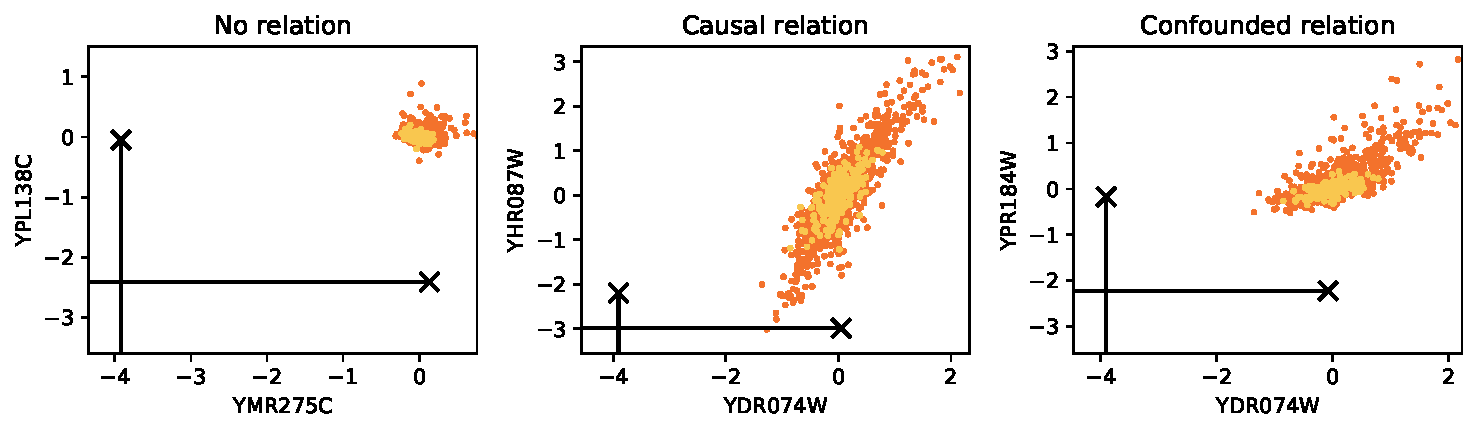
\includegraphics[width=\textwidth]{3gene_vs_gene}
    \caption{Expression levels of pairs of genes. All observation values are shown in orange, all intervention values in blue. The black crosses show the interventions on the plotted genes, the line shows which gene was intervened on.}
    \label{fig:3:genevsgene}
\end{figure}

\begin{figure}[h]
    \centering
    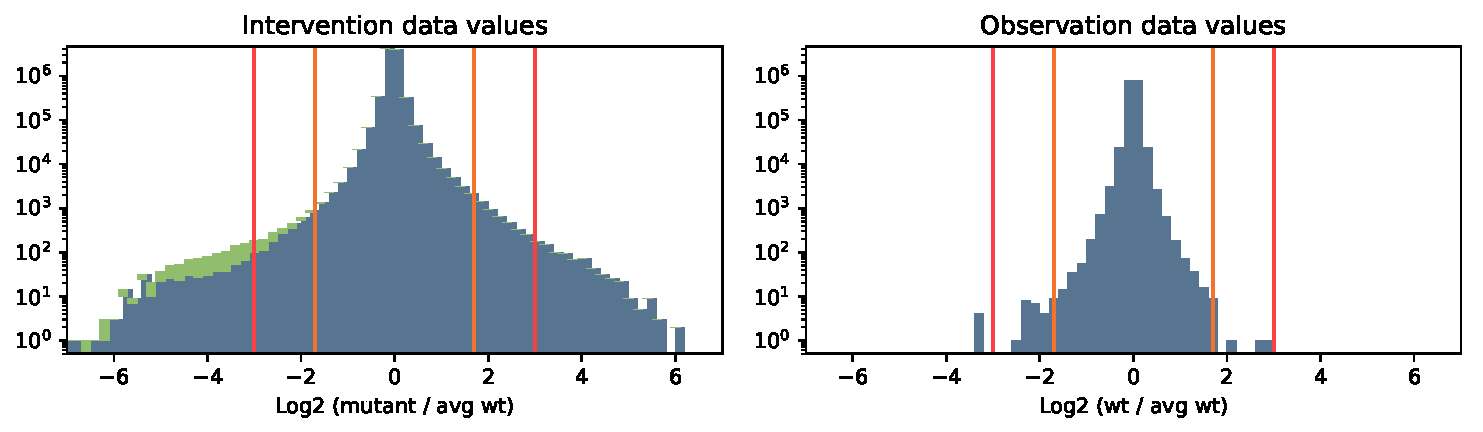
\includegraphics[width=\textwidth]{3data_values}
    \caption{Distribution of expression values in observation and intervention data. The values of the mutant genes themselves are shown in green. The ground-truth thresholds are shown in the intervention plot.}
    \label{fig:3:datavalues}
\end{figure}

\begin{figure}[h]
    \centering
    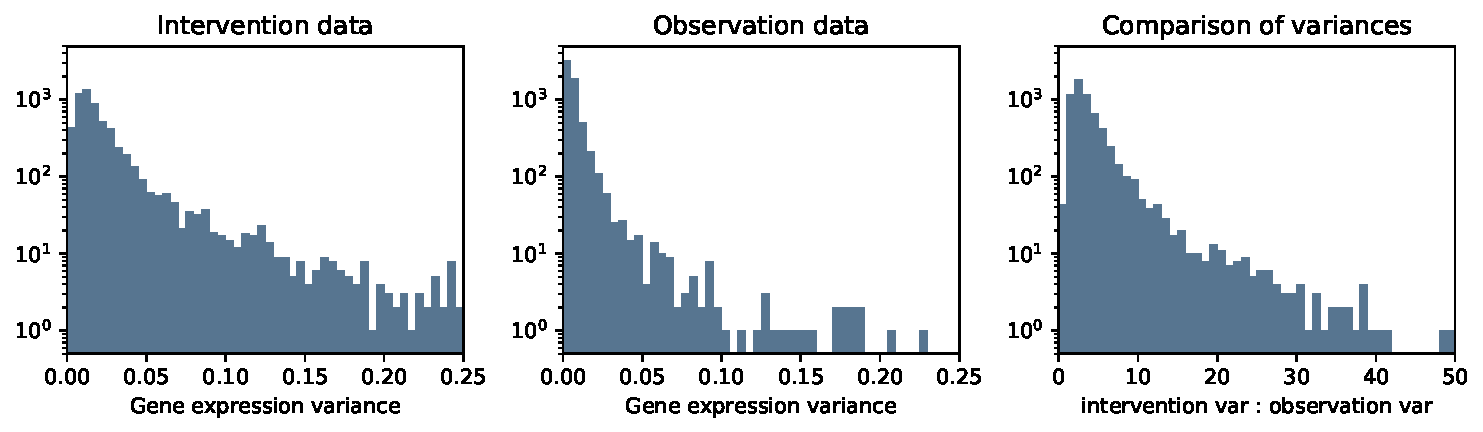
\includegraphics[width=\textwidth]{3gene_variance}
    \caption{Distribution of variance in the expression values of single genes in the observation and intervention data. The distribution of the ratio between intervention variance and observation variance per gene is shown on the right.}
    \label{fig:3:datavariance}
\end{figure}

Figure \ref{fig:3:genevsgene} shows examples of possible relations between two genes, distinguishing observation and intervention data. The relation between two variables can be visually estimated in these plots. In the middle plot, we see that the genes are correlated. By Reichenbach's principle we infer that there is some causal relation. Gene \textit{YHR087W} has reduced expression when we intervene on gene \textit{YDR074W}, but not the other way around. We may conclude that gene \textit{YDR074W} is an ancestor of gene \textit{YHR087W}. In the right plot we see two genes that are correlated, but do not respond to interventions. This indicates confounding.

Generally, the intervention data has higher \textbf{variance}, because the effect of the intervention propagates to many genes. Figure \ref{fig:3:datavalues} shows that the interventional data contains more extreme values. Figure \ref{fig:3:datavariance} compares the variance of genes in the observational and interventional data. In the interventional setting, the variance of genes tends to be about three, in some cases even more than ten times larger.

\begin{figure}[h]
    \centering
    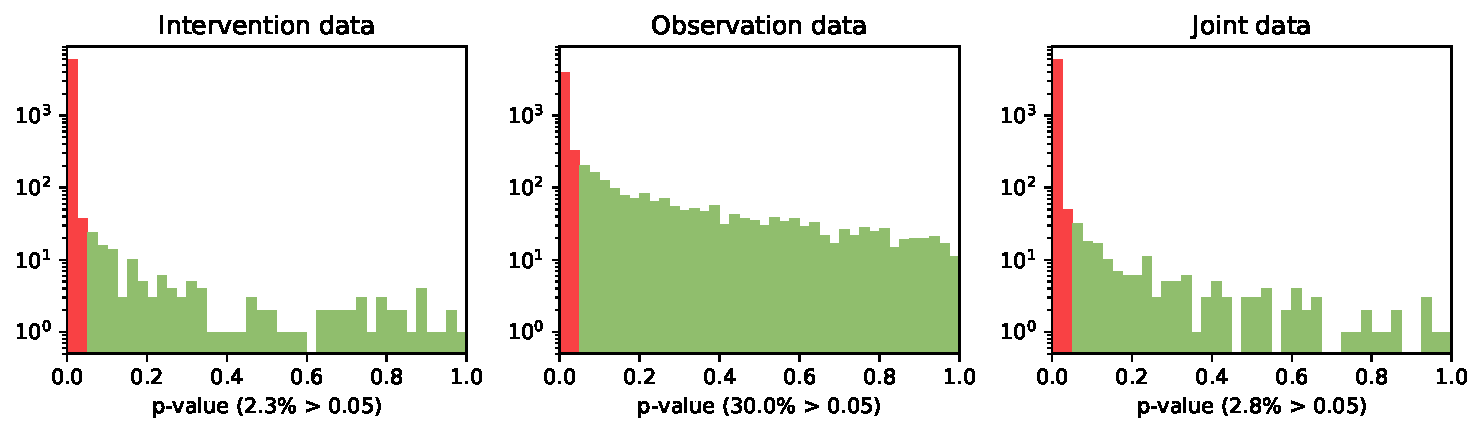
\includegraphics[width=\textwidth]{3normality}
    \caption{Distribution of p-values from the Shapiro-Wilk normality test per gene. For the intervention and joint data, we sampled 262 values per gene to make the p-values comparable.}
    \label{fig:3:normality}
\end{figure}   

The partial correlation test is commonly used in the causality literature to test if two variables are dependent or independent\footnote{When the test fails to reject the hypothesis of dependence, it is commonly concluded that the variables are dependent.} This test relies on the assumption that the data is \textbf{normally distributed}. Figure \ref{fig:3:normality} shows the results of a Shapiro-Wilk normality test. The normality assumption is more valid for the observational data than for the interventional data. This is to be expected, since we model the observational data to be sampled from a single distribution with some noise, and the interventional data from different distributions. Based on this test, visual inspection of the data as in Figure \ref{fig:3:genevsgene} and the general distribution of values in \ref{fig:3:datavariance}, we conclude that the normality assumption is acceptable. Nevertheless, different independence tests can still be interesting since they can capture other forms of independence. 

\begin{figure}[h]
    \centering
    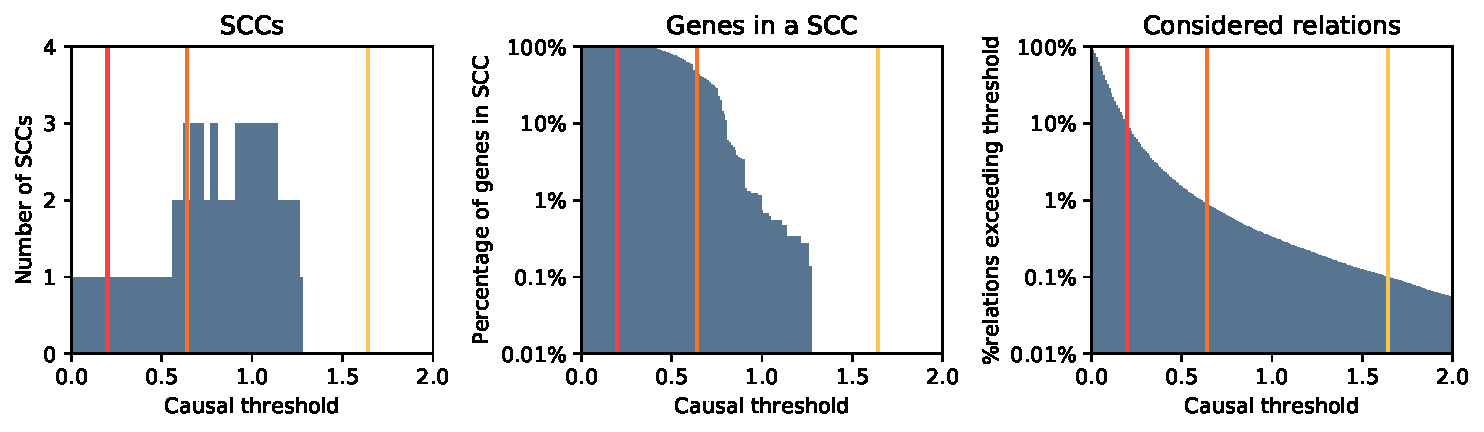
\includegraphics[width=\textwidth]{3cycles}
    \caption{Left: number of SCCs in the graph per ground-truth threshold. Middle: percentage of intervention genes that are in a SCC per threshold. Right: percentage of causal relations that are significant according to the threshold.}
    \label{fig:3:cycles}
\end{figure}    

Some causal inference methods, including our order-based LCD, assume that there are no \textbf{cycles} in the underlying graph. We construct a graph from the binary ground-truth and compute the number of strongly-connected components (SCCs): the number of variable subsets in which there is a directed path from each variable to each other variable. Combined with the number of variables in SCCs, this gives an indication of the validity of the acyclicity assumption. The results in Figure \ref{fig:3:cycles} show that for any ground-truth threshold, the number of SCCs is small. At the $1.7$ threshold, there are no SCCs and therefore no cycles. At the $1.0$ threshold, there are SCCs and only about $1\%$ of variables are in them. We conclude that acyclicity is an acceptable assumption, and it is a valid approach to search for a causal order of genes as a first step in our algorithm.

\begin{figure}[h]
    \centering
    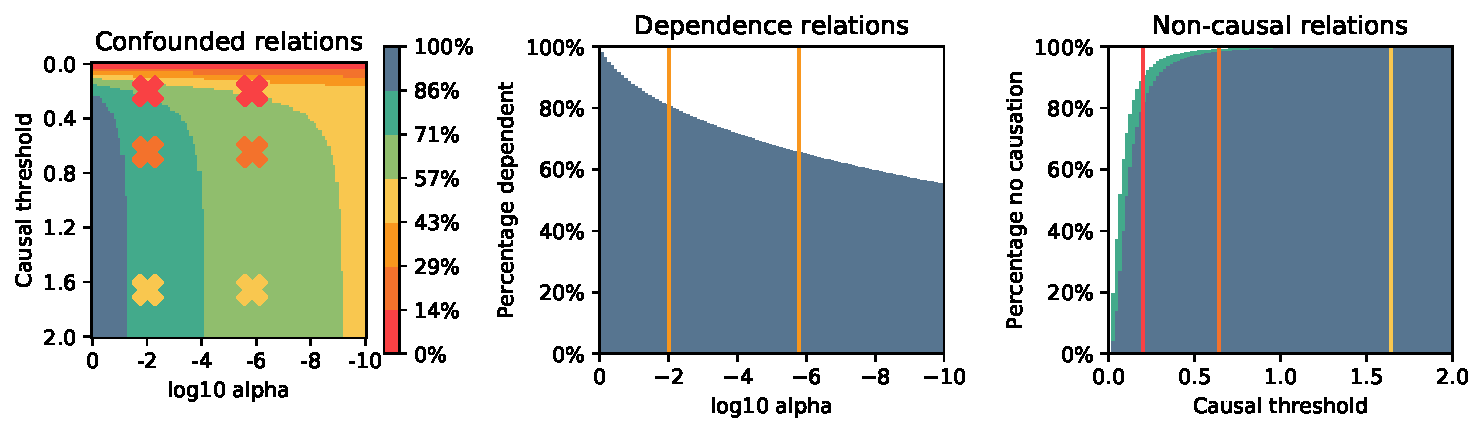
\includegraphics[width=\textwidth]{3confounding}
    \caption{Left: percentage of relations that are only related by confounding, for different binary thresholds, and significance levels. The two crosses show the alpha and thresholds used in this thesis. Middle: percentage of relations that are dependent per significance level. Right: percentage of relations that are not causal per binary ground-truth threshold (inverse of Figure \ref{fig:3:cycles}-right)}. Lighter color represents the knock-out values.
    \label{fig:3:confounding}
\end{figure}    

Next we test the frequency of \textbf{confounding} in the data. We could search for common ancestors in the binary ground-truth, but this will not find latent confounding. Therefore, we test for each variable pair if they are dependent (by the partial independence test), and not a cause of each other in the ground-truth. Note that we will miss variable pairs in which one variable causes another, while also being confounded. Figure \ref{fig:3:confounding} shows that at our ground-truth thresholds, and a significance level of $\alpha = \frac{1}{N} \approx 0.00057$, about $80\%$ of all relations among intervention genes is confounded. Note that both ground-truth thresholds are quite strict, so we mainly measure dependence among genes. We suspect that in the gene expressions are highly interconnected, explaining dependence between most genes. However, most of the relations are indirect and have relatively small effect, which makes it hard to infer the causal structure. Large prevalence of latent confounding is acceptable, since most methods can deal with it. However, the recall of LCD may be quite limited. It cannot identify ancestral relations that are also confounded, meaning that an expected $80\%$ of all relations are already disqualified.


\subsection{State-of-the-Art}

Due to the sparsity of the data, any kind of causal inference task is challenging. The few methods that have been applied on this data improve over some baseline only in a small number of strongest predictions. ICP is the method with the best performance. LCD has been tested as much faster alternative. Preselection is commonly used to speed up the algorithms, and might even improve accuracy of the most certain predictions. Three papers are shortly discussed in this subsection.

The ICP algorithm was first proposed by \textbf{\citet{peters2016causal}}, and tested on multiple datasets including the one of \citet{kemmeren2014large}. Two versions of ICP are designed, one with a test on regression coefficients, the other as faster alternative with an approximate test of residuals. L2-boosting regression \citep{schapire1998boosting} is used to preselect variables. Effects are considered true if the absolute intervention value exceeds the upper or lower $1\%$ of the observation values per gene, resulting in about $9.2\%$ of all effects being true. 6 out of the top 8 predictions of both ICP versions are true. A baseline that uses correlation on the pooled data has 2 true predictions in the top 8.

\textbf{\citet{meinshausen2016methods}} use ICP in a slightly different way, and evaluate against a different definition of true effects. They introduce a generalized ICP that accounts for latent confounding. They use stability selection \citep{meinshausen2010stability} to make a larger number of more fine-grained predictions, visualised in a receiver operating characteristic (ROC) curve. Effects are considered true only if the values of the cause and effect gene are extremes in the joint data, leading to a strict ground-truth set of about $0.1\%$ of all effects. The normal ICP version predicts 7 true effects in the first 9 predictions, and makes not one other true prediction in the top 25. The generalized ICP version predicts 5 true effects in the first 8 predictions and keeps making true predictions at a declining rate after that. A baseline using cross-validated sparse Lasso regression is provided for comparison, but it performs worse than random.

The most recent work on causal inference applied to the \citet{kemmeren2014large} dataset is by \textbf{\citet{versteeg2019boosting}}, who combine elements of both papers and investigate LCD as an alternative method that is faster. Predictions are made using stability selection. L2-boosting regression preselection is used for ICP and as an option for LCD. Two independence tests are compared, but no significant difference in performance is found. True effects are defined by the top $x\%$ absolute value in the intervention data. Methods are compared on a ROC curve, at ground-truth thresholds $10\%$, $1\%$, and $0.1\%$, but the comparative results are the same. In the first 100 predictions, ICP performs best, followed by LCD using preselection. An interesting result is that a baseline using only the preselection method outperforms the methods thereafter. LCD without preselection performs worse than this baseline from the start. ICP predicts about 40, 20, and 10 effects correctly in the first 100 for the respective ground-truth thresholds.

% \citet{tibshirani1996regression} Lasso regression

